\documentclass[titlepage]{article}
\usepackage[T1]{fontenc}
\usepackage[polish]{babel}
\usepackage[utf8]{inputenc}
\usepackage{amsmath}
\usepackage{graphicx}
\usepackage{titlepic}
\usepackage{url}


\author{Krzysztof Kulewski}
\title{Raspberry Pi}
\date{20.01.2016}
\titlepic{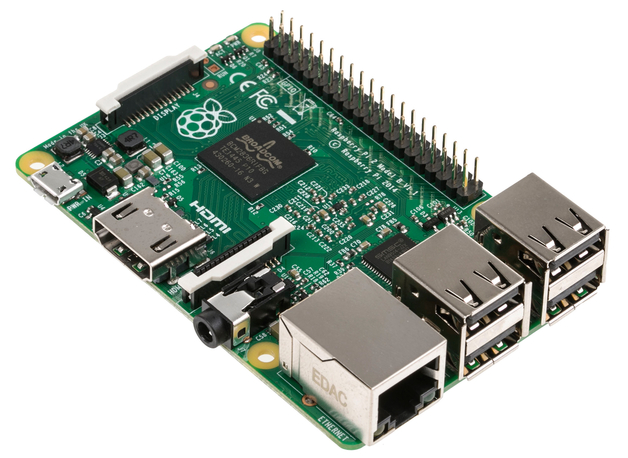
\includegraphics[width=\textwidth]{rpi2b.jpg}}


\begin{document}

\maketitle

\newpage

\tableofcontents

\newpage

\section{Wprowadzenie}
\subsection{Opis}
\textbf{Raspberry Pi} to komputer jednopłytkowy SBC, 
który został stworzony przez \textit{Raspberry Pi Foundation\cite{rpif}}.
Składa się z pojedynczego obwodu drukowanego, a jego premiera 
miała miejsce w I kwartale 2012 roku.

Urządzenie działa pod kontrolą systemów operacyjnych GNU/Linux i RISC OS oraz - w przypadku modelu Pi 2 B - również Windowsa 10 IoT.
Z założenia platforma miała przede wszystkim wspierać naukę 
podstaw informatyki, znalazła jednak szerokie zastosowanie w elektronice DIY, obok Arduino.
\\
Przykłady użycia:
\begin{itemize}
	\item przenośny PC
	\item serwer WWW - RPi z racji niewielkich rozmiarów oraz niskiego poboru prądu znakomicie sprawdza się w roli serwera
	\item robotyka - RPi może pełnić rolę głównego komputera
	\item automatyka domowa
	\item tablet (po zainstalowaniu wyświetlacza dotykowego)
	\item stacja pogodowa
	\item klaster
\end{itemize}
\subsection{Podstawowe modele}
Wyróżniamy kilka podstawowych wersji: 
\begin{enumerate}
	\item Pi 1 A (02.2012)
	\item Pi 1 B (05.2012)
	\item Pi 1 B+ (07.2014)
	\item Pi 1 A+ (11.2014)
	\item Pi 2 B (02.2015)
	\item Pi Zero (11.2015)
\end{enumerate}

\newpage



\section{Specyfikacja}
\subsection{Parametry wersji B oraz Zero}
Tabela \ref{table:parametry} na stronie \pageref{table:parametry} przedstawia parametry podstawowych modeli wersji B oraz Zero.

\begin{table}[!htb]
\begin{center}
\begin{tabular}{|c||l|l|l|l|}
% c - kolumna wycentrowana, l - wyjustowana do lewej
% r - wyjustowana do prawej
\hline  & Pi 1 B & Pi 1 B+ & Pi 2 B & Pi Zero \\ \hline \hline
Cena & 25\$ & 20\$ & 35\$ & 5\$ \\ \hline
SoC (Broadcom) & \multicolumn{2}{c|}{BCM2835} & BCM2836 & BCM2835 \\ \hline
CPU & \multicolumn{2}{c|}{700 MHz} & 900 MHz, quad & 1 GHz\\ \hline
GPU & \multicolumn{4}{c|}{Broadcom VideoCore IV @ 250 MHz}  \\ \hline
RAM & 256/512 MB & 512 MB & 1 GB & 512 MB \\ \hline
\end{tabular}
\caption{Parametry}
\label{table:parametry}
\end{center}
\end{table}

\subsection{Wyjścia wersji 2 B}
Grafika \ref{pic:rpi2b} przedstawia elementy Raspberry Pi 2 B.\cite{wiki}

\begin{figure}[!htb]
	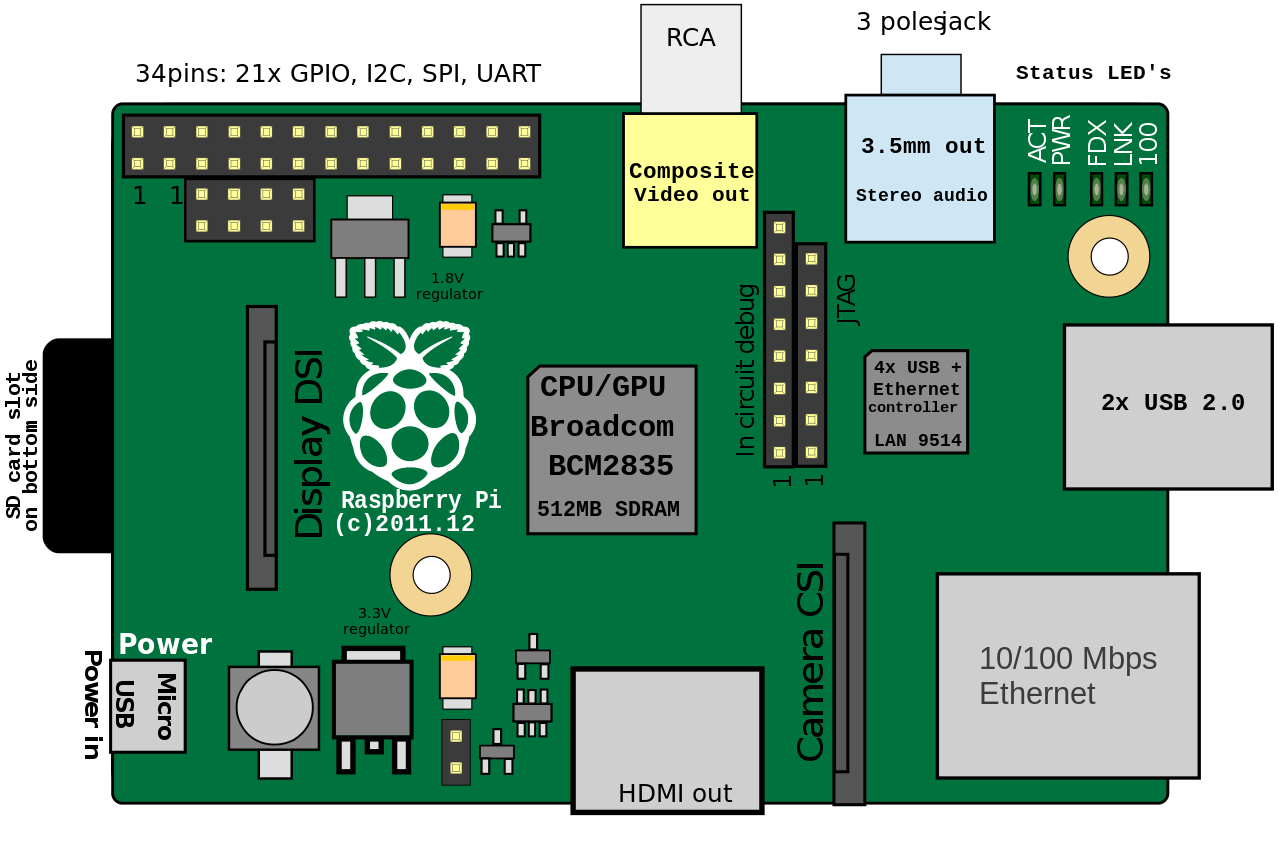
\includegraphics[scale=0.25]{pi2b_schema.png}
	\caption{Raspberry Pi 2 B}
	\label{pic:rpi2b}
\end{figure}

\newpage
\section{Wzory}
Poniższe wzory\cite{wz} mogą być użyteczne przy używaniu Raspberry Pi.
\subsection{Napięcie}
Wzór \ref{eq:volt} pozwala na obliczenie napięcia prądu elektrycznego.
\begin{equation}
\label{eq:volt} U = \Delta\varphi = \frac{W}{q}[V] 
\end{equation}

Gdzie:

$ U $ - napięcie prądu elektrycznego [V]

$ \Delta\varphi $ - różnica potencjałów [V]

$ W $ - praca [J]

$ q $ - przepływający ładunek [C]

\subsection{Natężenie}
Wzór \ref{eq:amp} pozwala na obliczenie natężenia prądu elektrycznego.
\begin{equation}
\label{eq:amp}
I = \frac{q}{t}[A]
\end{equation} 

Gdzie:

$ I $ - natężenie prądu [A]

$ q $ - przepływające ładunek

$ t $ - czas przepływu ładunku [s]

\subsection{Macierz}
Macierz modeli.

\begin{equation}
      M = \left[
        \begin{array}{cc}
         Pi B & Pi B+\\
         Pi 2 B & Pi Zero
         \end{array}
      \right]
      \qquad 
\end{equation}


\newpage
\begin{thebibliography}{99}
\bibitem{rpif} \url{http://www.raspberrypi.org/}
\bibitem{wiki} \url{https://en.wikipedia.org/wiki/Raspberry_Pi}
\bibitem{wz} Tablica wzorów fizycznych
\end{thebibliography}


\end{document}
